\documentclass{exam}
\usepackage[utf8]{inputenc}
\usepackage{lmodern}
\usepackage{microtype}

% \usepackage[parfill]{parskip}
\usepackage[dvipsnames]{xcolor}
\usepackage{amsmath}
\usepackage{amsfonts}
\usepackage{amsthm}
\usepackage{siunitx}
\DeclareSIUnit\year{yr}
\DeclareSIUnit\foot{ft}
\DeclareSIUnit\litre{\liter}

\usepackage{skull}

\usepackage{pgfplots}
\usepgfplotslibrary{polar}
\pgfplotsset{compat=1.11}
\usepgfplotslibrary{statistics}
\usepackage{graphicx}
\usepackage{sidecap}
\sidecaptionvpos{figure}{c}
\usepackage{float}
\usepackage{gensymb}
\usepackage{tkz-euclide}
\usetkzobj{all}
\usepackage{commath}
\usepackage{hyperref}
\usepackage{enumitem}
\usepackage{wasysym}
\usepackage{multicol}
\usepackage{mathtools}
\usepackage{tcolorbox}
\usepackage{tabularx}
\usepackage[version=4]{mhchem}
\usepackage{changepage}
\usepackage{listings}
\lstset{basicstyle=\ttfamily\linespread{0.8}\small}

\renewcommand*{\thefootnote}{\fnsymbol{footnote}}

\newtheorem*{thm}{Theorem}
\newtheorem*{iden}{Identity}
\newtheorem*{lemma}{Lemma}
\newtheorem{obs}{Observation}
\theoremstyle{definition}
\newtheorem*{defn}{Definition}
\newtheorem*{ex}{Example}
\newtheorem{con}{Construction}
\newtheorem*{alg}{Algorithm}

\newtheoremstyle{break}
  {\topsep}{\topsep}%
  {\itshape}{}%
  {\bfseries}{}%
  {\newline}{}%
\theoremstyle{break}
\newtheorem*{bthm}{Theorem}

% russian integral
\usepackage{scalerel}
\DeclareMathOperator*{\rint}{\scalerel*{\rotatebox{17}{$\!\int\!$}}{\int}}

% \DeclareMathOperator*{\rint}{\int}

\pgfplotsset{vasymptote/.style={
    before end axis/.append code={
        \draw[densely dashed] ({rel axis cs:0,0} -| {axis cs:#1,0})
        -- ({rel axis cs:0,1} -| {axis cs:#1,0});
    }
}}

% \pointsinrightmargin
\boxedpoints
\pointname{}

\newcommand{\questioA}{\question[\texttt{\textbf{\color{Cerulean} A}}]}
\newcommand{\questioM}{\question[\texttt{\textbf{\color{PineGreen} M}}]}
\newcommand{\questioE}{\question[\texttt{\textbf{\color{WildStrawberry} E}}]}
\newcommand{\questioS}{\question[\texttt{\textbf{\color{Goldenrod} S}}]}
\newcommand{\questioO}{\question[\texttt{\textbf{\color{BurntOrange} O}}]}

\newcommand{\parA}{\part[\texttt{\textbf{\color{Cerulean} A}}]}
\newcommand{\parM}{\part[\texttt{\textbf{\color{PineGreen} M}}]}
\newcommand{\parE}{\part[\texttt{\textbf{\color{WildStrawberry} E}}]}
\newcommand{\parS}{\part[\texttt{\textbf{\color{Goldenrod} S}}]}
\newcommand{\parO}{\part[\texttt{\textbf{\color{BurntOrange} O}}]}

\newcommand{\subparA}{\subpart[\texttt{\textbf{\color{Cerulean} A}}]}
\newcommand{\subparM}{\subpart[\texttt{\textbf{\color{PineGreen} M}}]}
\newcommand{\subparE}{\subpart[\texttt{\textbf{\color{WildStrawberry} E}}]}
\newcommand{\subparS}{\subpart[\texttt{\textbf{\color{Goldenrod} S}}]}
\newcommand{\subparO}{\subpart[\texttt{\textbf{\color{BurntOrange} O}}]}

\newcommand{\mainHeader}[2]{\section*{NCEA Level 2 Mathematics\\#1. #2}}
\newcommand{\mainHeaderHw}[2]{\section*{NCEA Level 2 Mathematics (Homework)\\#1. #2}}
\newcommand{\seealso}[1]{\begin{center}\emph{See also #1.}\end{center}}
\newcommand{\drills}[1]{\begin{center}\emph{Drill problems: #1.}\end{center}}
\newcommand{\basedon}[1]{\begin{center}\emph{Notes largely based on #1.}\end{center}}

\begin{document}

\mainHeaderDiffHw{7}{The Geometry of Functions}
\subsection*{Reading}
The `proper' name for the subject we are beginning to look at now is \emph{differential geometry}. One of the pioneers of this
subject was Leonhard Euler.

\begin{center}
  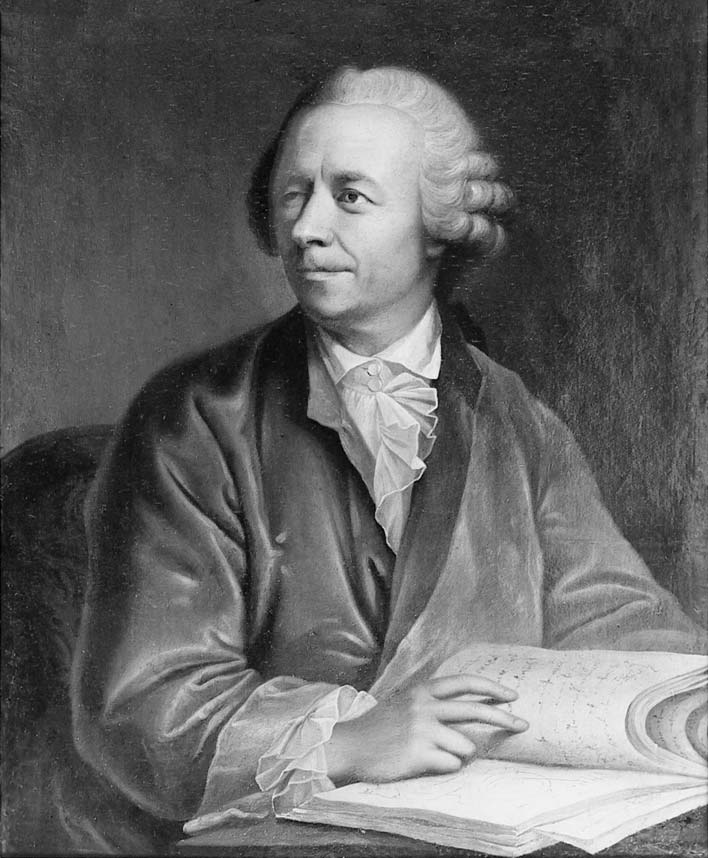
\includegraphics[width=0.2\textwidth]{euler}
\end{center}

Leonhard Euler (1707--1783) was Switzerland's foremost scientist and one of the three greatest mathematicians of modern times (the other two being
Gauss and Riemann).

He was perhaps the most prolific author of all time in any field. From 1727 to 1783 his writings poured out in a seemingly endless flood, constantly
adding knowledge to every known branch of pure and applied mathematics, and also to many that were not known until he created them. He averaged about
800 printed pages a year throughout his long life, and yet he almost always had something worthwile to say and never seems long-winded. The publication
of his complete works was started in 1911, and the end is not in sighr: it is now esitmated that 100 large volumes will be required for completion
of the project. He suffered blindess during the last 17 years of his life, but with the aid of his powerful memory and fertile imagination, and with
helpers to write his books and papers from dictation, he actually increased the already prodigious output of work.

Though he was not himself a teacher Euler has had a deeper influence on the teaching of mathematics than any other person. This came about chiefly
through his three great treatises: \emph{Introductio in Analysin Infinitorum} (1748); \emph{Institutiones Calculi Differentialis} (1755);
and \emph{Institutiones Calculi Integralis} (1768--1794). There is considerable truth in the old saying that all elementary and advanced calculus
textbooks since 1748 are essentially copies of Euler or copies of copies of Euler. These works summed up and codified the discoveries of his
predecessors, and are full of Euler's own ideas. He extended and perfected plane and solid analytic geometry, introduced the analytic approach
to trigonometry, and was responsible for the modern treatment of the functions $ \ln $ and $ \exp $. It was though his work that the symbols $ e $,
$ \pi $, and $ i $ became common currency for all mathematicians, as well as the functions $ \sin $ and $ \cos $.

He was the first and greatest master of infinite series, products, and fractions; in 1736, he made the wonderful discovery that
\begin{displaymath}
  1 + \frac{1}{4} + \frac{1}{9} + \frac{1}{16} + \cdots = \frac{\pi^2}{6},
\end{displaymath}
and also found the sums of the reciprocals of the fourth and sixth powers. (A closed form for the sum of the reciprocals of the
cubes is still unknown.)

The foundations of classical mechanics had been laid down by Newton, but Euler was the principle architect. In his treatise of 1736
he was the first to explicitly introduce the concept of a point-like particle, and he was the also the first to study the acceleration
of a particle moving along any curve and to use the notion of a vector in connection with velocity and acceleration. His continued
successes in mathematical physics were so numerous, and his influence was so pervasive, that most of his discoveries are not credited
to him at all and are taken for granted by physicists as part of the natural order of things.

\begin{flushright}
  Adapted from \textit{Differential equations with applications and historical notes} (pp.136--146) by George F. Simmons (McGraw-Hill, 1991).
\end{flushright}

\clearpage
\subsection*{Questions}
\begin{questions}
  \question Explain, with sketches, the geometric meaning of the second derivative.
  \question Find the second derivative of the following functions.
    \begin{parts}
      \part $ f(x) = x^5 - 5x + 3 $
      \part $ f(x) = \frac{x^2}{x - 1} $
      \part $ f(x) = \sqrt{x} - \sqrt[4]{x} $
    \end{parts}
  \question Sketch a function satisfying the given criteria.
    \begin{parts}
      \part (hint: your result should be an odd function)
        \begin{subparts}
           \subpart $ f'(1) = f'(-1) = 0 $,
           \subpart $ f'(x) < 0 $ if $ \abs{x} < 1 $,
           \subpart $ f'(x) > 0 $ if $ 1 < \abs{x} < 2 $,
           \subpart $ f'(x) = -1 $ if $ \abs{x} > 2 $.
        \end{subparts}
      \part
        \begin{subparts}
          \subpart $ f'(x) < 0 $,
          \subpart $ f''(x) < 0 $.
        \end{subparts}
    \end{parts}
\end{questions}
\end{document}
